\newpage

\mainmatter
\pagenumbering{arabic}
\chapter{Foundation of Mathematics}

For this chapter, we would like to give a brief introduction to (General Relativity)GR's mathematical foundation. At the beginning of the development of GR, the researcher tried hard to seek for a mathematical language to describe curved spacetime. Concepts in topology, including \textbf{manifolds}, are exposed to play a role in general relativity. Therefore, starting from fundamental mathematical concepts is much essential for us.

\newpage

\section{Manifold}
Just think of a balloon, children always like to blow up a balloon. We can observe the behavior of the balloon itself and find that it quietly looks like our universe in inflation. If we want to describe the surface of a balloon traditional Euclidean geometry is inconvenient for us. Also, people are used to looking at flat maps, because the earth is so large relative to us that we can almost think of the ground below us as a flat surface. Therefore, to describe the surface of the Earth, we can use many maps to approximate the local area, which can roughly meet our daily needs, and this idea of describing a curved surface (such as the Earth) corresponds to a very practical mathematical structure, the manifold. But we can't introduce manifolds directly in this section, because we lack several concepts before defining manifolds. Then we start from the basic thing: \textbf{Topology}. 

\textbf{In this section, we needn't spend much time in mathematical form. Try to understand the motivation we introduce the concept of manifolds.}

\subsection{Topology}

First, to know how small area can be considered as "local area" that is flat area we should consider its nature of neighborhood, that is 

\begin{tcolorbox}[title=\textbf{Neighborbood},colback=SeaGreen!10!CornflowerBlue!10,colframe=RoyalPurple!55!Aquamarine!100!]
    A \textbf{neighborhood} is a of points that are "close" to a given point. 
\end{tcolorbox}

How you define what "proximity" means depends on the topological space you're dealing with, but neighborhoods have some definite characteristics. Dealing with neighborhoods directly can be annoying, so we use open subsets instead.

What is a subset? It's kind of abstract for us because it is difficult to imagine any kind of open subset. Generally speaking, it's just a rule for a set to specify which subsets are open subsets and so on.

\begin{tcolorbox}[title=\textbf{Open Subsets},colback=SeaGreen!10!CornflowerBlue!10,colframe=RoyalPurple!55!Aquamarine!100!]
    Consider a set $X$, we define open subsets as 
    \begin{itemize}
        \item $X$ itself and empty set are open subsets
        \item The intersection of finite open subsets is open subset
        \item The union of arbitrary numbers of open subsets(or infinite open subsets) is open subset
    \end{itemize}
\end{tcolorbox}

And for any rule that satisfy above requirements in set $X$ is called \textbf{topological structure}. And all the open subset in $X$ that has defined topological structure also compose a set is called \textbf{topology}, denoted as $\mathscr{T}$. We also use $\mathscr{P}$ to represent all the subsets of $X$. 

With three rules about open subsets, the study of spatial structure can be simplified.

\subsection{Charts and Atlases}

With the definition of open subsets, we can know what a "local area" is. Similar with a map for a given area, actually the map can not directly describe surface in earth, because the map is flat and the surface of earth is curved. So, we should construct a relationship between a group of points in map and corresponding points in the surface of earth. That is called a \textbf{Chart}.

\begin{tcolorbox}[title=\textbf{Charts},colback=SeaGreen!10!CornflowerBlue!10,colframe=RoyalPurple!55!Aquamarine!100!]
    The chart is a diagram map from an open subset of a manifold to an open subset of a Euclidean space.
\end{tcolorbox}
 
Obviously, Euclidean space is corresponding to a flat map, and an open subset of a manifold is an area in the surface on the earth. 

\begin{figure}[htbp]
    \centering
    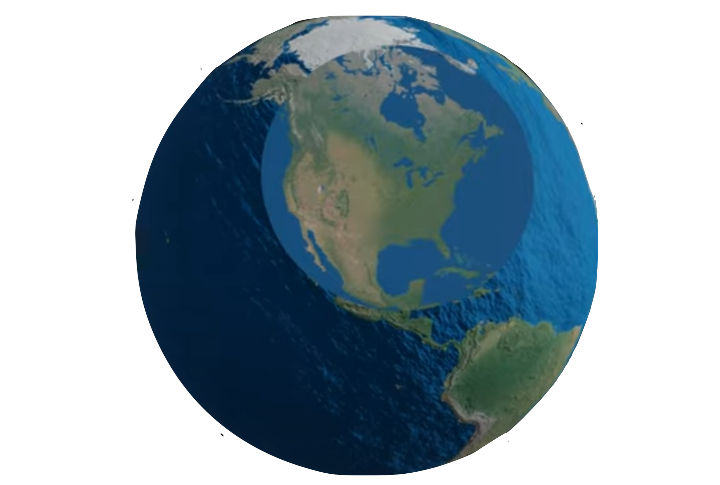
\includegraphics[width=6cm]{pic/earth.png}
    \caption{We take an area to transform a flat map}
\end{figure}

From these statements, we can conclude some properties of manifolds. First, from a practical point of view, we need Euclidean space to conveniently describe what we care about. So this leads us to think about the relationship between Euclidean space and a manifold. Combined with the neighborhood we talk about before, a manifold should be a mathematical structure that conforms locally to the description of Euclidean space. And we use charts to describe such local nature that is the same as a map for a certain country. 

\begin{figure}[htbp]
    \centering
    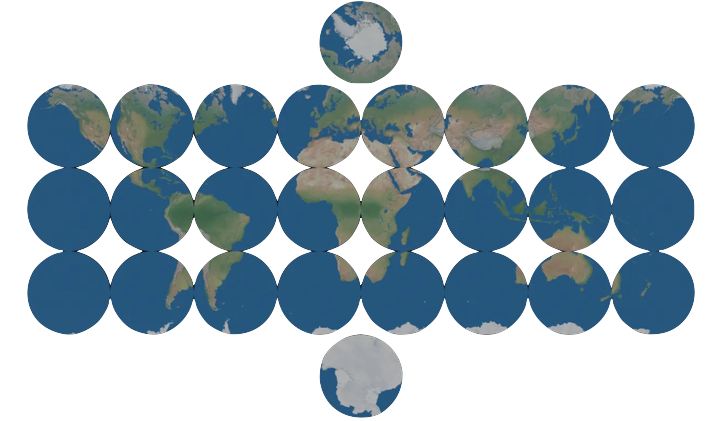
\includegraphics[width=8cm]{pic/earths.png}
    \caption{After we take lots of charts and we can know all information of the earth}
\end{figure}

Therefore, we need more charts to cover it. Each chart is a function mapped from a part of a manifold to a Euclidean space. By grouping many of these charts together, we can cover the entire manifold. This is the concept of an atlas, which is a set of charts that cover the entire manifold. Therefore, in order to describe the entire manifold, we need at least one chart to cover each point, and together these charts form an \textbf{atlas}.

To cover the entire manifold we can design a group of charts that don't overlap with each other. But it's not necessary for us because such mathematical structure is much inconvenient. We allow overlap and just think of the area overlapped. To avoid conflicts, we need claim that any two chart cover the same point that it should exist a way from one chart to another chart. Such transformation is called \textbf{transition map}. 

It is easy to understand it. Just like sewing a football with cloth, we need several pieces of cloth to make a ball, which can also overlap the cloth. Obviously, there is always a way to match the dots on two pieces of cloth that correspond to the same position in the overlapping area. 

\begin{figure}[htbp]
    \centering
    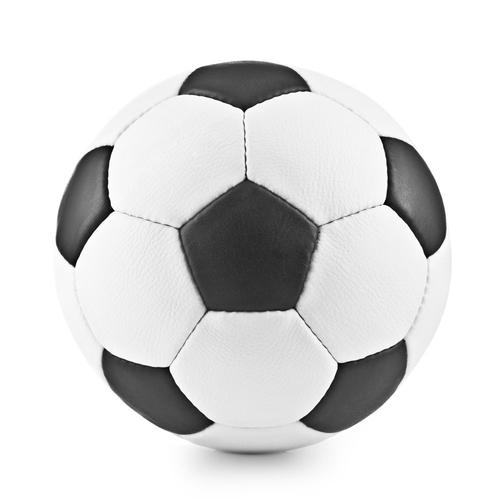
\includegraphics[width=5cm]{pic/football.jpeg}
    \caption{Please focus on the clothes on the surface of such football.}
\end{figure}

\subsection{Manifolds}

In mathematics, a manifold is a topological space that locally resembles Euclidean space near each point. Manifolds can be equipped with additional structures. One important class of manifolds is differentiable manifolds; their differentiable structure allows calculus to be done.

In principle, transition maps can be anything, but we always want to place some restrictions on them. A transition map is said to be \textbf{differentiable} if it has derivatives everywhere. Having a differentiable manifold means that the space is locally similar enough to a vector space that we can perform derivative operations on it. \textbf{If we can take any number of derivatives of a transition map, we say that the manifold is smooth.}

Then I would like to give an example to show what is a manifold.

\begin{tcolorbox}[title=\textbf{Circle},colback=SeaGreen!10!CornflowerBlue!10,colframe=RoyalPurple!55!Aquamarine!100!]
    A circle is the simplest example of a topological manifold. Topology ignores bending, so a small piece of a circle is treated the same as a small piece of a line. This corresponds to the fact that manifolds locally represent Euclidean space.

    Obviously, a circle can't be represented by single chart because chart is an open set, which you can't put end to end. So we need to find two or more charts to cover a circle. 

    Such functions along with the open regions they map are called charts. Similarly, there are charts for the bottom (red), left (blue), and right (green) parts of the circle:

    \begin{align*}
        \chi_{top}(x,y)=x\\
        \chi_{left}(x,y)=y\\
        \chi_{bottom}(x,y)=y\\
        \chi_{right}(x,y)=x
    \end{align*}
    Together, these parts cover the whole circle, and the four charts form an atlas for the circle.
\end{tcolorbox}

\begin{figure}[htbp]
    \centering
    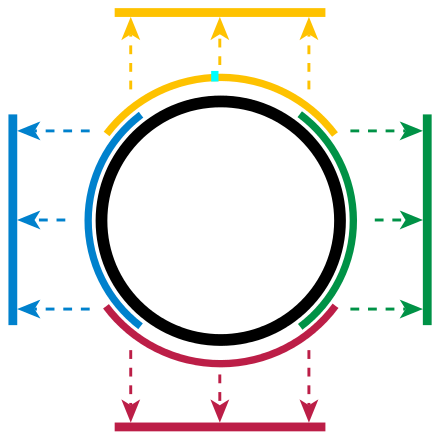
\includegraphics[width=6cm]{pic/circle.png}
    \caption{The four charts each map part of the circle to an open interval, and together cover the whole circle.}
\end{figure}

If you ask us to use several words to describe what is manifold, I'll give you such words:

\begin{itemize}
    \item Local Euclidean space
    \item Covering
    \item Smooth(For differentiable manifolds)
\end{itemize}


\section{Scalar, Vector, Tensor}

\subsection{Vector Space and Vector}

Based on the differentiable manifolds, the transition map is differentiable that we can introduce more mathematical structure like vector space.

Let's go back to linear algebra, and review the concept of vector space.

\begin{tcolorbox}[title=\textbf{Vector Space},colback=SeaGreen!10!CornflowerBlue!10,colframe=RoyalPurple!55!Aquamarine!100!]
    A vector space over a field of real numbers is a set attached with two kinds of map, addition: $V\times V\rightarrow V$ and scalar multiplication: $\mathbb{R}\times V\rightarrow V$, which satisfy:
    \begin{itemize}
        \item $v_{1}+V_{2}=v_{2}+v_{1}, \quad \forall v_{1},v_{2}\in V;$
        \item $(v_{1}+v_{2})+v_{3}=v_{1}+(v_{2}+v_{3}),\quad \forall v_{1},v_{2},v_{3}\in V$;
        \item \exists\, (Zero element) $\underline{0}\in V$ let \,$\underline{0}+v=v, \quad \forall v\in V$;
        \item $\alpha_{1}(\alpha_{2} v )=(\alpha_{1}+\alpha_{2})v,\quad  \forall v\in V, \alpha_{1},\alpha_{2}\in \mathbb{R} $;
        \item $(\alpha_{1}+\alpha_{2})v=\alpha_{1}v+\alpha_{2}v, \quad \forall v\in V,\alpha_{1}, \alpha_{2} \in \mathbb{R}$;
        \item $\alpha(v_{1}+v_{2})=\alpha v_{1}+\alpha v_{2},\quad \forall v_{1},v_{2}\in V, \alpha \in \mathbb{R}$;
        \item 1\cdot v=v, 0\cdot v=0, \quad v\in V.
    \end{itemize}
\end{tcolorbox}

We are already familiar with the inference of vector space, and we can not directly define the vector in manifolds. So we need to use more general mathematical language to define it.

\begin{tcolorbox}[title=\textbf{Vector},colback=SeaGreen!10!CornflowerBlue!10,colframe=RoyalPurple!55!Aquamarine!100!]
    A map $v:\mathscr{F}_{M}\rightarrow \mathbb{R}$ is defined as a \textbf{vector} in point $p\in M$, if $\forall f,g,\in \mathscr{F}_{M}, \alpha,\beta\in \mathbb{R}$:
    \begin{itemize}
        \item (Linearity) $v(\alpha f+\beta g)= \alpha v(f)+\beta v(g)$;
        \item (Leibniz's law) $v(fg)=f|_{p}v(g)+g|_{p}v(f)$,  where $f|_{p}$ represents value of function $f$ in point $p$, denoted as $f(p)$.
    \end{itemize}
\end{tcolorbox}

How to understand this map? It differs from our conventional concept that a vector is just a bar with an arrow which implies two key elements: length and direction. However, when we switch to the general point of view, we need to summarize its essence, this map is to tell us a point in the manifold corresponds to a real number. The map is arbitrary, so there are countless vectors corresponding to countless maps. If we know the local area in point $p$ is mapping a Euclidean space, then we can construct a map from Euclidean space to a vector that we can certainly describe this vector. What else, you can see this map that it acts on a function and meanwhile, it leads us to introduce the \textbf{coordinates} and \textbf{basis} to describe it.

\subsection{Coordinate and basis}

Recall the concept of coordinates, we can use several numbers to describe location of a point(relatively). Of course, the kind of coordinate is countless, we should select more convenient one in given situations. Also, whatever we choose, it should contains the same information for us. That is to say, we can change coordinate system, but we can not get new physics.

For example, we want to describe an ant on a ball. It's obvious to select spherical coordinate to describe its location, motion and so on. Here we are, set the radius of ball is $r$. There exists a limitation $r^{2}=x^{2}+y^{2}+z^{2}$. So the freedom degree is two, we can just use two sets of number to describe it.

\begin{align}
    X=\sin \theta\cos \phi\\
    Y=r\sin \theta\sin \phi\\
    Z=r\cos\theta
\end{align}

For this instance, coordinates $(r,\theta,\phi)$ and $(X,Y,Z)$ are both effective. Generally speaking, we denote $(x_{1},x_{2},\cdots,x_{n})$ as generalized coordinate. 

Then with definition of coordinate, we can also define what is curve. Just like a ball

\begin{tcolorbox}[title=\textbf{Curve},colback=SeaGreen!10!CornflowerBlue!10,colframe=RoyalPurple!55!Aquamarine!100!]
    Set $I$ is an interval, so $C^{r}$ map defined as $C:I\rightarrow M$ is called a curve on the manifold $M$. For any $t\in I$, it corresponds unique point $C(t)\in M$, called \textbf{parameter}.
\end{tcolorbox}

It differs from our traditional definition, when we think of the curve it usually corresponds subsets in manifold $M$. Actually, curve is map itself. So if we select another parameter but also map the same subset, we assume they are different. 




\subsection{Tangent Vector}

If we have a coordinate system $(O,\Psi)$ and coordinate $x^{\mu}$. Then as for any smooth function $f\in \mathscr{F}_{M}$ we use such coordinate system to generate a N-element function $F(x^{1},\cdots, x^{n})$, which implies a group of vector denoted as $X_{\mu}$ that act on a function $f\in \mathscr{F}_{M}$ resulting a real number $X_{\mu}(f)$:

\begin{align}
    X_{\mu}(f):=\left.\frac{\partial F(x^{1},\cdots, x^{n})}{\partial x^{\mu}}\right|_{p}, \quad \forall f\in \mathscr{F}_{M}
\end{align}

And any vector $v$ can be linearly represented by the form of 

\begin{align}
    v=v^{\mu}X_{\mu}
\end{align}

where 

\begin{align}
    v^{\mu}=v(x^{\mu})
\end{align}

Summarize it, and we can get the definition of coordinate basis 

\begin{tcolorbox}[title=\textbf{Coordinate},colback=SeaGreen!10!CornflowerBlue!10,colframe=RoyalPurple!55!Aquamarine!100!]
    For a point $p$ in the field of manifold, $\{X_{1},\cdots,X_{n}\}$ is called $V_{p}$'s \textbf{coordinate basis}. 
    Every $X_{\mu}$ is called a \textbf{coordinate basis vector}. And the value $v^{\mu}$ resulted by linear representation of $v\in V_{p}$ with $\{X_{\mu}\}$ is called $v$'s \textbf{coordinate components}.
\end{tcolorbox}

Obviously, we use many kinds of coordinates, and many physical essences is found in transformation of coordinate. Given that two coordinates $\{x^{\mu}\}, \{x^{\prime\nu}\}$, and the intersection of two fields of coordinate is not null. And we select one point located at the intersection, $v\in V_{p}$, $\{v^{\mu}\},\{v^{\prime \nu}\}$ is coordinate components for $v$ under two coordinates, we have


\begin{align}
    v^{\prime \nu}=\left.\frac{\partial x^{\prime \nu}}{\partial x^{\mu}}\right|_{p}v^{\mu}
\end{align}

The above equation is called \textbf{Vector component transformation expression}.

\subsection{Dual Vector}


We also need to introduce another kind of vector called \textbf{dual vector}. Since called "vector", it also has linearity and Leibniz law. However, what is different from normal vectors is that it constructs a kind of map from vectors to real numbers. Give an example, here we have a simple equation "\textbf{one} plus \textbf{two} equals three"

\begin{align}
    \mathbbb{1}+\mathbbb{2}=3\in \mathbb{R}\label{add}
\end{align}

Obviously, for a single number, we can consider it a "vector", and it satisfies the calculation rules of the vector. Now we need "create" a new kind of number called "dual number" with an adder. That is to say, Eq. \ref{add} can be divided into two categories: "number" and "dual number". And dual number itself also has the same Linearity and Leibniz law. And it has such a calculation rule: acts on a number and get a real number. That is the key point of dual vector.

\begin{align}
    \underset{Dual Number}{\boxed{\mathbbb{1}+}}\;\underset{Number}{\mathbbb{2}}=3\in \mathbb{R}
\end{align}

We give the definition of dual vector space 

\begin{tcolorbox}[title=\textbf{Dual Vector Space},colback=SeaGreen!10!CornflowerBlue!10,colframe=RoyalPurple!55!Aquamarine!100!]
    The dual space is the space of all linear maps from the original vector space to the real numbers; in math lingo, if $\omega\in T_{p}^*$  is a dual vector, then it acts as a map such that
    \begin{align}
        \omega(aV+bW)=a\omega (V)+b\omega (W)\in \mathbb{R}\label{def:dual}
    \end{align}
\end{tcolorbox}

On the basis of Def. \ref{def:dual}, we know the definition of dual vector is based on acting on vectors, so we also need to construct them with coordinate basis vector. Therefore, we can derive dual vector basis by acting on vector basis.
\begin{align}
    \hat{e}^{(\mu)}\hat{e}_{(\nu)}=\delta^{(\mu)}_{(\nu)}
\end{align}

So a dual vector can be expressed by basis
\begin{align}
    A=A^{\mu}\hat{e}_{(\mu)}
\end{align}

In the view of Dirac formalism, we can get the same form, but what is mostly different from with above "vector" is the spaces that they live are different. For Dirac formalism, the vector also can be expressed by 
\begin{align}
    \ket{\psi}=\sum_{i=1}^{n}A_{i}\ket{i}
\end{align}
For dual vector basis, we have
\begin{align}
    \braket{j}{i}=\delta^{j}_{i}.
\end{align}
Thus, dual vector has
\begin{align}
    \bra{\psi'}=\sum^{n}_{j=1}B_{j}\bra{j}
\end{align}.
Therefore, we can find that the definition of dual space in much common for physics.


